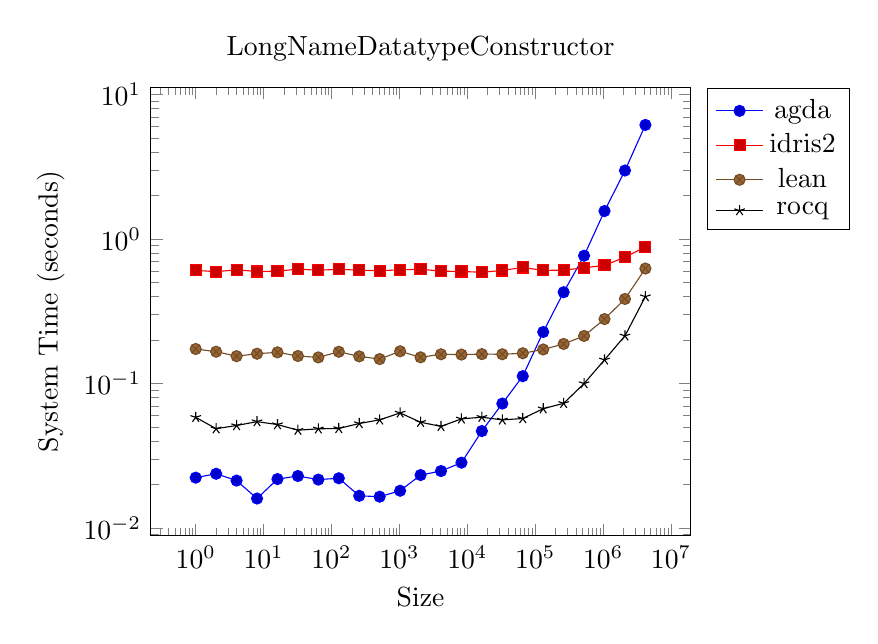
\begin{tikzpicture}
\begin{loglogaxis}
[title=LongNameDatatypeConstructor,
xlabel={Size},
ylabel={System Time (seconds)},
legend entries={agda,idris2,lean,rocq},
legend pos=outer north east,
]\addplot coordinates {
(4194304.0,6.17737) [0]
(2097152.0,2.985575) [0]
(1048576.0,1.564812) [0]
(524288.0,0.767548) [0]
(262144.0,0.428868) [0]
(131072.0,0.227418) [0]
(65536.0,0.112434) [0]
(32768.0,7.2645e-2) [0]
(16384.0,4.6871e-2) [0]
(8192.0,2.8307e-2) [0]
(4096.0,2.4773e-2) [0]
(2048.0,2.3235e-2) [0]
(1024.0,1.8091e-2) [0]
(512.0,1.6453e-2) [0]
(256.0,1.6687e-2) [0]
(128.0,2.2081e-2) [0]
(64.0,2.1612e-2) [0]
(32.0,2.2886e-2) [0]
(16.0,2.1794e-2) [0]
(8.0,1.5979e-2) [0]
(4.0,2.127e-2) [0]
(2.0,2.3716e-2) [0]
(1.0,2.2292e-2) [0]
};
\addplot coordinates {
(4194304.0,0.882717) [0]
(2097152.0,0.749762) [0]
(1048576.0,0.65837) [0]
(524288.0,0.633115) [0]
(262144.0,0.609649) [0]
(131072.0,0.607411) [0]
(65536.0,0.636715) [0]
(32768.0,0.607112) [0]
(16384.0,0.589273) [0]
(8192.0,0.597262) [0]
(4096.0,0.599797) [0]
(2048.0,0.619279) [0]
(1024.0,0.612787) [0]
(512.0,0.604328) [0]
(256.0,0.608754) [0]
(128.0,0.618164) [0]
(64.0,0.608709) [0]
(32.0,0.620022) [0]
(16.0,0.599727) [0]
(8.0,0.59681) [0]
(4.0,0.613249) [0]
(2.0,0.595057) [0]
(1.0,0.607773) [0]
};
\addplot coordinates {
(4194304.0,0.625748) [0]
(2097152.0,0.385158) [0]
(1048576.0,0.279469) [0]
(524288.0,0.21355) [0]
(262144.0,0.188019) [0]
(131072.0,0.172073) [0]
(65536.0,0.162008) [0]
(32768.0,0.159481) [0]
(16384.0,0.159844) [0]
(8192.0,0.15863) [0]
(4096.0,0.159397) [0]
(2048.0,0.151876) [0]
(1024.0,0.167197) [0]
(512.0,0.147726) [0]
(256.0,0.154163) [0]
(128.0,0.165925) [0]
(64.0,0.151666) [0]
(32.0,0.155103) [0]
(16.0,0.164408) [0]
(8.0,0.160878) [0]
(4.0,0.154659) [0]
(2.0,0.166085) [0]
(1.0,0.173425) [0]
};
\addplot coordinates {
(4194304.0,0.3998) [0]
(2097152.0,0.213921) [0]
(1048576.0,0.145893) [0]
(524288.0,9.9916e-2) [0]
(262144.0,7.2926e-2) [0]
(131072.0,6.6924e-2) [0]
(65536.0,5.7247e-2) [0]
(32768.0,5.5977e-2) [0]
(16384.0,5.8435e-2) [0]
(8192.0,5.6898e-2) [0]
(4096.0,5.0476e-2) [0]
(2048.0,5.3946e-2) [0]
(1024.0,6.2567e-2) [0]
(512.0,5.6047e-2) [0]
(256.0,5.2834e-2) [0]
(128.0,4.8851e-2) [0]
(64.0,4.8561e-2) [0]
(32.0,4.7515e-2) [0]
(16.0,5.1965e-2) [0]
(8.0,5.4459e-2) [0]
(4.0,5.1203e-2) [0]
(2.0,4.8633e-2) [0]
(1.0,5.8357e-2) [0]
};
\end{loglogaxis}
\end{tikzpicture}
